\renewcommand{\teacherTag}{QUESTION 6 \textbullet\ 35 MARKS}
\chapter{Convolution, Causality and Stability}

%------------------------------------------------------------------ 6(a)
\begin{qcard}{Q6(a)}{Discrete convolution with a step}{17}
Let $0<\alpha<1$. Consider $x[n]=\alpha^nu[n]$ and $h[n]=u[n]$. Compute the convolution $y[n]=x[n]*h[n]$ and show that
\[y[n]=\frac{1-\alpha^{n+1}}{1-\alpha}\,u[n].\]
Also sketch $y[n]$.
\end{qcard}
\begin{solution}
\step{Step 1 --- Definition.}
\[y[n]=\sum_{k=-\infty}^{\infty}x[k]\,h[n-k]=\sum_{k=-\infty}^{\infty}\alpha^ku[k]\;u[n-k].\]
\step{Step 2 --- Find where the terms are non-zero.} $u[k]=1$ needs $k\ge0$; $u[n-k]=1$ needs $k\le n$. (Graphically: $h[n-k]$ is the step flipped about $k=0$ and slid to $k=n$; it covers $k\le n$.)
\begin{center}
\begin{tikzpicture}
\begin{axis}[width=12cm,height=3.8cm,axis lines=middle,xlabel={$k$},xmin=-4.6,xmax=8.6,ymin=0,ymax=1.35,xtick={-4,...,8},ytick=\empty,ticklabel style={font=\scriptsize},label style={font=\scriptsize},legend style={font=\scriptsize,draw=none,at={(0.5,1.04)},anchor=south,legend columns=2}]
\addplot+[ycomb,navy,thick,mark=*,mark size=1.6pt]coordinates{(0,1)(1,0.6)(2,0.36)(3,0.216)(4,0.13)(5,0.078)(6,0.047)(7,0.028)(8,0.017)};\addlegendentry{$x[k]=\alpha^ku[k]$}
\addplot+[ycomb,coral,thick,mark=square*,mark size=1.4pt,xshift=2pt]coordinates{(-4,1.1)(-3,1.1)(-2,1.1)(-1,1.1)(0,1.1)(1,1.1)(2,1.1)(3,1.1)(4,1.1)};\addlegendentry{$h[n-k]$ for $n=4$}
\fill[gold,opacity=0.18](axis cs:-0.4,0)rectangle(axis cs:4.4,1.3);
\node[font=\scriptsize,anchor=south]at(axis cs:2,1.12){overlap $0\le k\le n$};
\end{axis}
\end{tikzpicture}
\end{center}
\begin{itemize}[leftmargin=1.4em,itemsep=2pt]
\item $n<0$: no overlap (the step ends at $k=n<0$ before $x$ starts), so $y[n]=0$.
\item $n\ge0$: the overlap is $0\le k\le n$.
\end{itemize}
\step{Step 3 --- Sum the geometric series} (first term 1, ratio $\alpha\ne1$, $n+1$ terms):
\[y[n]=\sum_{k=0}^{n}\alpha^k=\frac{1-\alpha^{n+1}}{1-\alpha},\qquad n\ge0 .\]
Combining both cases:
\[\boxed{y[n]=\frac{1-\alpha^{n+1}}{1-\alpha}\,u[n]}\]
\step{Step 4 --- Behaviour.} $y[0]=1$, $y[1]=1+\alpha$, $y[2]=1+\alpha+\alpha^2$, \dots: convolving with $u[n]$ is a running sum (accumulator). Since $0<\alpha<1$, $\alpha^{n+1}\to0$ and $y[n]$ rises monotonically to the limit $\dfrac1{1-\alpha}$.
\begin{center}
\begin{tikzpicture}
\begin{axis}[width=12cm,height=5cm,axis lines=middle,xlabel={$n$},ylabel={$y[n]$},xmin=-3.6,xmax=12.6,ymin=0,ymax=2.9,xtick={-3,...,12},ytick={1,1.6,2.5},yticklabels={$1$,$1+\alpha$,$\frac1{1-\alpha}$},ticklabel style={font=\scriptsize},label style={font=\scriptsize}]
\addplot+[ycomb,navy,thick,mark=*,mark size=1.6pt,samples at={0,...,12}]{(1-0.6^(x+1))/(1-0.6)};
\addplot+[ycomb,navy,thick,mark=*,mark size=1.6pt]coordinates{(-3,0)(-2,0)(-1,0)};
\addplot[dashed,crimson,domain=-0.5:12.6]{2.5};
\node[font=\scriptsize,crimson,anchor=south east]at(axis cs:12.4,2.52){limit $1/(1-\alpha)$};
\end{axis}
\end{tikzpicture}
\end{center}
\begin{notebox}The sketch is drawn for $\alpha=0.6$, so $y[0]=1$, $y[1]=1.6$, $y[2]=1.96$, \dots, $y[\infty]=2.5$. The shape is the same for every $0<\alpha<1$: zero for $n<0$, starts at 1, increases monotonically, saturates at $\frac1{1-\alpha}$.\end{notebox}
\ans{$y[n]=\sum_{k=0}^n\alpha^k=\dfrac{1-\alpha^{n+1}}{1-\alpha}u[n]$; it starts at $1$ and rises monotonically to $\dfrac1{1-\alpha}$.}
\end{solution}

%------------------------------------------------------------------ 6(b)
\begin{qcard}{Q6(b)}{Causality and stability of three systems}{6 + 6 + 6}
For each continuous-time LTI system determine whether it is causal and whether it is stable. Justify your answers.
\[\text{(i) } h_1(t)=e^{-3t}u(2-t)\qquad\text{(ii) } h_2(t)=e^{-5\abs t}\qquad\text{(iii) } h_3(t)=te^{-2t}u(t)\]
\end{qcard}
\begin{solution}
\begin{keyidea}For an LTI system: \textbf{causal} $\iff h(t)=0$ for all $t<0$; \textbf{BIBO stable} $\iff\int_{-\infty}^{\infty}\abs{h(t)}\dd t<\infty$.\end{keyidea}

\step{(i) $h_1(t)=e^{-3t}u(2-t)$.} $u(2-t)=1$ for $t\le2$, so $h_1$ lives on $(-\infty,2]$.
\begin{itemize}[leftmargin=1.4em,itemsep=2pt]
\item Causal? $h_1(-1)=e^{3}\ne0$: non-zero for negative time $\Rightarrow$ \textbf{not causal}.
\item Stable? $\displaystyle\int_{-\infty}^{2}e^{-3t}\dd t=\Big[-\tfrac13e^{-3t}\Big]_{-\infty}^{2}=-\tfrac13e^{-6}+\tfrac13\lim_{t\to-\infty}e^{-3t}=\infty$ (the exponential \emph{grows} as $t\to-\infty$) $\Rightarrow$ \textbf{not stable}.
\end{itemize}
\step{(ii) $h_2(t)=e^{-5\abs t}$.} A two-sided decaying exponential.
\begin{itemize}[leftmargin=1.4em,itemsep=2pt]
\item Causal? $h_2(t)=e^{5t}\ne0$ for $t<0$ $\Rightarrow$ \textbf{not causal}.
\item Stable? $\displaystyle\int_{-\infty}^\infty e^{-5\abs t}\dd t=2\int_0^\infty e^{-5t}\dd t=\frac25<\infty$ $\Rightarrow$ \textbf{stable}.
\end{itemize}
\step{(iii) $h_3(t)=te^{-2t}u(t)$.}
\begin{itemize}[leftmargin=1.4em,itemsep=2pt]
\item Causal? $u(t)$ makes $h_3=0$ for $t<0$ $\Rightarrow$ \textbf{causal}.
\item Stable? $h_3\ge0$, and $\displaystyle\int_0^\infty te^{-2t}\dd t=\frac{1!}{2^2}=\frac14<\infty$ (by parts, or $\int_0^\infty t^ne^{-at}=\frac{n!}{a^{n+1}}$) $\Rightarrow$ \textbf{stable}. The factor $t$ grows only linearly; the exponential decay wins.
\end{itemize}
\begin{center}
\begin{tikzpicture}\begin{axis}[width=5.3cm,height=3.6cm,axis lines=middle,xlabel={$t$},title={(i) $e^{-3t}u(2-t)$},xmin=-1.6,xmax=3,ymin=0,ymax=5,xtick={-1,2},ytick=\empty,ticklabel style={font=\scriptsize},label style={font=\scriptsize},title style={font=\scriptsize}]
\addplot[very thick,crimson,domain=-1.6:2,samples=60]{exp(-3*x)};\addplot[very thick,crimson]coordinates{(2,0.0025)(2,0)(3,0)};
\end{axis}\end{tikzpicture}
\begin{tikzpicture}\begin{axis}[width=5.3cm,height=3.6cm,axis lines=middle,xlabel={$t$},title={(ii) $e^{-5\abs t}$},xmin=-1.5,xmax=1.5,ymin=0,ymax=1.25,xtick={-1,1},ytick={1},ticklabel style={font=\scriptsize},label style={font=\scriptsize},title style={font=\scriptsize}]
\addplot[very thick,coral,domain=-1.5:1.5,samples=121]{exp(-5*abs(x))};
\end{axis}\end{tikzpicture}
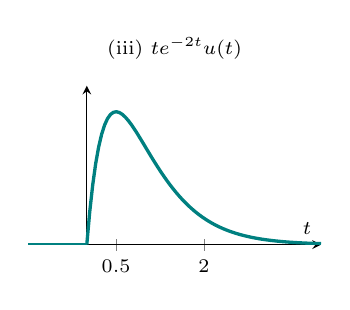
\begin{tikzpicture}\begin{axis}[width=5.3cm,height=3.6cm,axis lines=middle,xlabel={$t$},title={(iii) $te^{-2t}u(t)$},xmin=-1,xmax=4,ymin=0,ymax=0.22,xtick={0.5,2},ytick=\empty,ticklabel style={font=\scriptsize},label style={font=\scriptsize},title style={font=\scriptsize}]
\addplot[very thick,teal,domain=0:4,samples=80]{x*exp(-2*x)};\addplot[very thick,teal]coordinates{(-1,0)(0,0)};
\end{axis}\end{tikzpicture}
\end{center}
\begin{center}\small\renewcommand{\arraystretch}{1.3}\begin{tabular}{@{}lccl@{}}\toprule
system&causal&stable&reason\\\midrule
(i) $e^{-3t}u(2-t)$&no&no&non-zero for $t<0$; grows as $t\to-\infty$\\
(ii) $e^{-5\abs t}$&no&yes&non-zero for $t<0$; $\int\abs h=\frac25$\\
(iii) $te^{-2t}u(t)$&yes&yes&zero for $t<0$; $\int\abs h=\frac14$\\\bottomrule\end{tabular}\end{center}
\ans{(i) neither causal nor stable; (ii) stable but not causal ($\int\abs{h}=\frac25$); (iii) causal and stable ($\int\abs{h}=\frac14$).}
\end{solution}
